\section*{Aufgabe 4 (26 Punkte)}
\vspace{0.4cm}
\subsection*{\frage{1}{3}}
Geben ist die Funktion
\begin{align*}
f \ : \ \mathbb{R}^2_{++} \to \mathbb{R}^2_{++},
\ \
(x,y) \mapsto f(x,y) = (x^2 + 2\ x \ y + y^2) e^{x+y}. 
\end{align*}
Ihre partiellen Elastizitäten $ \varepsilon_{f,x}(x,y) $ und
$ \varepsilon_{f,y}(x,y) $ genügen der Ungleichung
\renewcommand{\labelenumi}{(\alph{enumi})}
\begin{enumerate}
	\item 
	$ \varepsilon_{f,x} > \varepsilon_{f,y}  $ für alle $ (x,y) \in \mathbb{R}^2_{++} $.
	\item
	$ \varepsilon_{f,x} < \varepsilon_{f,y}  $ für alle $ (x,y) \in \mathbb{R}^2_{++} $.
	\item
	$ \varepsilon_{f,x} < \varepsilon_{f,y}  $ für $ (x,y) \in \mathbb{R}^2_{++} $ mit $ x > y $.
	\item
	$ \varepsilon_{f,x} < \varepsilon_{f,y}  $ für $ (x,y) \in \mathbb{R}^2_{++} $ mit $ x < y $.
\end{enumerate}
\ \\
\textbf{Lösung:}
\begin{mdframed}
\underline{\textbf{Vorgehensweise:}}
\renewcommand{\labelenumi}{\theenumi.}
\begin{enumerate}
\item Berechne die partiellen Ableitungen von $ f $.
\item Finde die korrekte Antwort.
\end{enumerate}
\end{mdframed}

\underline{1. Berechne die partiellen Ableitungen von $ f $}\\
Zuerst verwenden wir die erste binomische Formel und erhalten 
\begin{align*}
f(x,y) = (x^2 + 2xy + y^2) e^{x+y} = (x+ y)^2 e^{x+y}.
\end{align*}
Mit der Produktregel \& Kettenregel folgt 
\begin{align*}
f_x(x,y)
&= 2(x + y) e^{x+y} + (x+y)^2 e^{x+y}
= (2(x+y) +(x+y)^2) e^{x+y}\\
f_y(x,y) &= 2(x + y) e^{x+y} + (x+y)^2 e^{x+y} = (2(x+y) +(x+y)^2) e^{x+y},
\end{align*}
dass $ f_x(x,y) = f_y(x,y) $ gilt. Durch
\begin{align*}
\varepsilon_{f,x} &= x \frac{f_x(x,y)}{f(x,y)}\\
\varepsilon_{f,y} &= y \frac{f_y(x,y)}{f(x,y)}
\end{align*}
können wir die Antworten (a) und (b) direkt ausschließen.
\\
\\
\underline{2. Finde die korrekte Antwort}\\
Wir wissen bereits, dass $ f_x(x,y) = f_y(x,y) $ gilt und $ f $ strikt positiv ist. Damit folgt 
\begin{align*}
f_x(x,y) = f_y(x,y) \ \Rightarrow \
\frac{f_x(x,y)}{f(x,y)} = \frac{f_y(x,y)}{f(x,y)}
\end{align*}
und falls $ x < y $ ist, erhalten wir
\begin{align*}
x \frac{f_x(x,y)}{f(x,y)} < y\frac{f_y(x,y)}{f(x,y)}.
\end{align*}
Damit gilt $ \varepsilon_{f,x} < \varepsilon_{f,y}  $ für $ (x,y) \in \mathbb{R}^2_{++} $ mit $ x < y $.\\
\\
Die Antwort (d) ist korrekt.
\newpage

\subsection*{\frage{2}{4}}

\renewcommand{\labelenumi}{(\alph{enumi})}
Gegeben ist die Funktion
\begin{align*}
f \ : \ \mathbb{R} \to \mathbb{R}_{++}, \ \ 
x \mapsto f(x) = x^2 \ e^{x^2} + 1
\end{align*}
\begin{enumerate}
	\item 
	$ f $ hat ein lokales Maximum in $ x_0 = 0 $.
	\item
	$ f $ hat ein lokales Minimum in $ x_0 = 0 $.
	\item
	$ f $ hat einen Wendepunkt in $ x_0 = 0 $.
	\item
	$ f $ hat keine stationären Punkte.
\end{enumerate}
\ \\
\textbf{Lösung:}
\begin{mdframed}
\underline{\textbf{Vorgehensweise:}}
\renewcommand{\labelenumi}{\theenumi.}
\begin{enumerate}
\item Überlege dir argumentativ, welche Antwort korrekt ist.
\item Alternativer Lösungsweg. 
\end{enumerate}
\end{mdframed}

\underline{1. Überlege dir argumentativ, welche Antwort korrekt ist}\\
Die Funktion $ f $ setzt sich aus $ x^2 $ und $ e^{x^2} $ zusammen.
Die Verschiebung um $ 1 $ auf der $ y $-Achse spielt keine Rolle bei Extrempunkten. Der Term $ x^2 $ besitzt ein Minimum in $ x_0 = 0 $. Die Exponentialfunktion ist streng monoton wachsend, d.h.
es gilt
\begin{align*}
x < y \ \Rightarrow \ e^x < e^y.
\end{align*}
Dementsprechend nimmt auch der Term $ e^{x^2}  $ sein Minimum in $ x_0 = 0 $ an. Also ist Antwort (b) korrekt.\\
\\
\underline{2. Alternativer Lösungsweg}\\
Es gilt
\begin{align*}
f^\prime(x) = 2 x e^{x^2} + x^2 2 x e^{x^2} = 2x e^{x^2} ( 1 + x^2)
\end{align*}
mithilfe der Produkt \& Kettenregel.
Wegen $ e^{x^2} ( 1 + x^2)  > 0$ für alle $ x \in \mathbb{R} $ erhalten wir durch
\begin{align*}
f^\prime(x) = 0 \ \Leftrightarrow \ 
2x e^{x^2} ( 1 + x^2) = 0
\
\Leftrightarrow
\
x = 0
\end{align*}
den stationären Punkt $ x_0 = 0 $. 
%Aufgrund des Terms $ 2x $ ist dieser mit
%\begin{align*}
%f^\prime(x) < 0 \ &\text{für} \ x < 0 \\
%f^\prime(x) > 0 \ &\text{für} \ x > 0
%\end{align*}
%ein Minimum.
%Alternativ lässt sich dies auch mit der zweiten Ableitung begründen.
Es handelt sich um ein Minimum, da $ f^{\prime \prime}(0) > 0 $ gilt. Dies werden wir nun durch Ermittlung der zweiten Ableitung nachweisen. Es gilt
%\begin{align*}
%f^\prime(x) = 2 e^{x^2}(x + x^3),
%\end{align*}
%woraus
\begin{align*}
f^{\prime \prime}(x)
&=
2 ( 2x e^{x^2} (x + x^3)  + 2 e^{x^2} (1 + 3 x^2 ))
=
2 ( 2 e^{x^2} (x^2 + x^4) + 2  e^{x^2} ( 1 + 3 x^2))\\
&=
2  e^{x^2} ( 2 x^4  + 3x^3 +  2x^2   + 1)
\
\Rightarrow
\
f^{\prime \prime}(0) = 2 \cdot 1 > 0
\end{align*}
mithilfe der Produkt \& Kettenregel.
Damit besitzt $ f $ in $ x_0 = 0  $ ein Minimum.
\newpage
\subsection*{\frage{3}{4}}
Gegeben ist die Funktion
\begin{align*}
f \ : \ D_f  \to \mathbb{R}, x \mapsto f(x) = \frac{1}{1+x}.
\end{align*}
$ P_3 $ und $ P_4 $ seien die Taylorpolynome dritter und vierter Ordnung von $ f $ in $ x_0 = 0 $.\\
\\
Dann gilt:
\renewcommand{\labelenumi}{(\alph{enumi})}
\begin{enumerate}
	\item 
	$ P_3(x) > P_4(x) $ für alle $ x \in D_f \setminus \{ x_0\} $.
	\item
	$ P_3(x) < P_4(x) $ für alle $ x \in D_f \setminus \{ x_0\} $.
	\item
	$ P_3(x) = P_4(x) $ für alle $ x \in D_f \setminus \{ x_0\} $.
	\item
	Jeder der Fälle $ P_3(x) > P_4(x) $, $ P_3(x) < P_4(x) $ oder $ P_3(x) = P_4(x) $ ist für entsprechende $ x \in D_f \setminus \{ x_0\} $ möglich.
\end{enumerate}
\ \\
\textbf{Lösung:}
\begin{mdframed}
\underline{\textbf{Vorgehensweise:}}
\renewcommand{\labelenumi}{\theenumi.}
\begin{enumerate}
\item Stelle das vierte Taylorpolynom mithilfe von $ P_3 $ dar und überlege, was du hieraus schließen kannst.
\end{enumerate}
\end{mdframed}

\underline{1. Stelle das vierte Taylorpolynom mithilfe von $ P_3 $ dar und überlege, was du hieraus schließen kannst}\\
Im Allgemeinen lässt sich sagen, dass
\begin{align*}
P_4(x) = P_3(x) + \frac{f^{(4)}(0)}{4!} x^4
\end{align*}
gilt. Wegen $ x^4  > 0 $ für $ x \in D_f \setminus \{ x_0\} $, ist die korrekte Antwort abhängig vom Vorzeichen von $ f^{(4)}(0) $.
Dies können wir durch 
\begin{align*}
&P_3(x) = P_4(x)
\ \Leftrightarrow \
 \frac{f^{(4)}(0)}{4!} x^4 = 0
\ \Leftrightarrow \
f^{(4)}(0) = 0\\
&P_3(x) < P_4(x)
\ \Leftrightarrow \
 \frac{f^{(4)}(0)}{4!} x^4 > 0
\ \Leftrightarrow \
f^{(4)}(0) > 0\\
&P_3(x) > P_4(x)
\ \Leftrightarrow \
 \frac{f^{(4)}(0)}{4!} x^4 <0
\ \Leftrightarrow \
f^{(4)}(0) < 0\\
\end{align*}
formalisieren. Da $ f^{(4)}(0) $ konstant ist, können wir Antwort (d) bereits ausschließen.
Des Weiteren liefert uns die Struktur der Ableitungen von $ f $, dass $ f^{(4)}(0) $ positiv ist. Dies sehen wir daran, dass gerade Ableitungen in $ x_0 = 0 $ immer positiv sind. Damit können wir hier schon sagen, dass Antwort (b) korrekt ist.
Dies wollen wir aber noch durch
\begin{align*}
f^\prime(x) &=
-1 (x+1)^{-2}
=
 - \frac{1}{(x+1)^2} \quad
f^{\prime \prime}(x) = 
(-1) \cdot (-2)  \cdot (x + 1 )^{-3}
=
\frac{2}{(x+1)^3}\\
f^{\prime \prime \prime}(x) &= 
2 \cdot(-3) (x+1)^{-4}
=
- \frac{6}{(x+1)^4}\\
f^{(4)}(x) &= 
(-4) \cdot (-6) \cdot (x+1)^{-5}
=
\frac{24}{(x+1)^5}
\ \Rightarrow \
f^{(4)}(0) = 24 > 0
\end{align*}
untermauern. Damit ist Antwort (b) korrekt.

\newpage
\subsection*{\frage{4}{4}}
Gegeben sind die Funktionen
\begin{align*}
f(x,y) = \sqrt{1 - 4  x^2 - y^2}
\end{align*}
und
\begin{align*}
g(x,y)
= 
\ln(2  x - x^2 - y^2 + 8) 
\end{align*}
mit den entsprechenden Definitionsgebieten $ D_f $ und $ D_g $.\\
\\
Dann gilt:
\renewcommand{\labelenumi}{(\alph{enumi})}
\begin{enumerate}
	\item 
	$ D_f \subseteq D_g $.
	\item
	$ D_g \subseteq D_f $.
	\item
	$ D_f = D_g $.
	\item
	$ D_f \cap D_g = \emptyset $.
\end{enumerate}
\ \\
\textbf{Lösung:}
\begin{mdframed}
\underline{\textbf{Vorgehensweise:}}
\renewcommand{\labelenumi}{\theenumi.}
\begin{enumerate}
\item Stelle die Definitionsbereiche von $ f $ und $ g $ durch geometrische Objekte dar.
\end{enumerate}
\end{mdframed}

\underline{1. Stelle die Definitionsbereiche von $ f $ und $ g $ durch geometrische Objekte dar}\\
Für den Definitionsbereich von $ f $ muss die Gleichung
\begin{align*}
1 - 4x^2 -y^2 \geq 0
\
\Leftrightarrow
\
4x^2 + y^2 \leq 1
\ \Leftrightarrow \
\frac{x^2}{\left(\frac{1}{2}\right)^2} + \frac{y^2}{1^2} \leq 1
\ \Leftrightarrow \
x \in D_f
\end{align*}
erfüllt sein.
Hierdurch wird eine Ellipsenfläche mit den Halbachsen $ a = \frac{1}{2}$, $ b = 1 $ und dem Mittelpunkt $ (0,0) $ beschrieben.\\ \\
Für den Definitionsbereich von $ g $ muss die Gleichung
\begin{align*}
2x - x^2 -y^2 + 8 > 0
&\ \Leftrightarrow \
x^2 - 2x + y^2 < 8
\ \Leftrightarrow \
x^2 - 2x + 1 - 1 + y^2 < 8\\
&\ \Leftrightarrow \
(x-1)^2 + y^2 < 9 =3^2
\ \Leftrightarrow \
x \in D_g
\end{align*}
erfüllt sein. Hierdurch wird eine Kreisfläche mit Mittelpunkt $ (1,0) $ und dem Radius $ 3 $ dargestellt.
Insgesamt erhalten wir mit
\begin{align*}
(x \in D_f \ \Rightarrow \ x \in D_g)  \ \Leftrightarrow \ (D_f \subseteq D_g)
\end{align*}
die korrekte Antwort (b). Dies können wir auch durch folgende Grafik veranschaulichen:
\begin{center}
	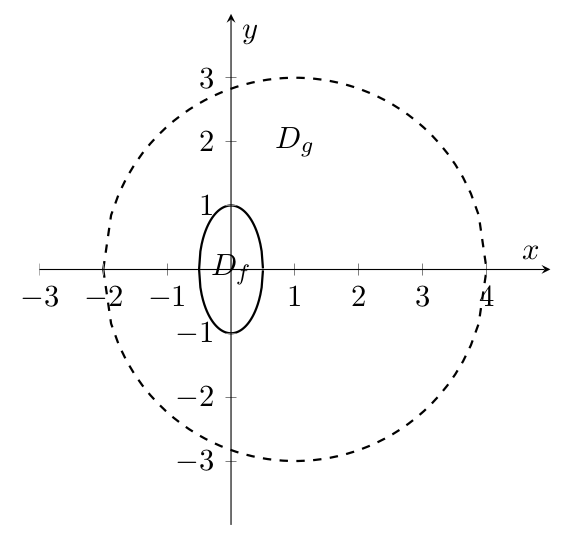
\includegraphics[width=0.3\textwidth]{pictures/auf4_4.png}
\end{center}
\newpage

\subsection*{\frage{5}{3}}
Sei $ f(x) = \sin(x) $ und $ P_3  $ das Taylorpolynom  dritter Ordnung von $ f $ in $ x_0 = 0 $.\\
\\
Welche der folgenden Aussagen bezüglich des Restglieds dritter Ordnung $ R_3 $ von $ f  $ in $ x_0 = 0 $ ist wahr?
\renewcommand{\labelenumi}{(\alph{enumi})}
\begin{enumerate}
	\item 
	$ |R_3(x)| \leq \frac{|x|^4}{128} $ für alle $ x \in \mathbb{R} $.
	\item
	$ |R_3(x)| \leq \frac{|x|^4}{64} $ für alle $ x \in \mathbb{R} $.
	\item
	$ |R_3(x)| \leq \frac{|x|^4}{32} $ für alle $ x \in \mathbb{R} $.
	\item
	$ |R_3(x)| \leq \frac{|x|^4}{16} $ für alle $ x \in \mathbb{R} $.
\end{enumerate}
\ \\
\textbf{Lösung:}
\begin{mdframed}
\underline{\textbf{Vorgehensweise:}}
\renewcommand{\labelenumi}{\theenumi.}
\begin{enumerate}
\item Betrachte die Definition des Restglieds dritter Ordnung in $ x_0 = 0 $ von $ f $ und leite die korrekte Antwort her.
\item 
Alternativer Lösungsweg.
\end{enumerate}
\end{mdframed}

\underline{1. Betrachte die Definition des Restglieds dritter Ordnung in $ x_0 = 0 $ von $ f $ \\ und leite die korrekte Antwort her}\\
Das Restglied dritter Ordnung von $ f $ in $ x_0 = 0 $ ist durch
\begin{align*}
R_3(x)
= 
\frac{f^{(4)}(\xi)}{4!} x^4
\end{align*}
definiert.
Es gilt 
\begin{align*}
f^\prime(x) &= \cos(x)\\
f^{\prime \prime}(x) &= - \sin(x)\\
f^{\prime \prime \prime}(x) &= - \cos(x)\\
f^{(4)}(x) &= \sin(x) 
\ \Rightarrow \
| f^{(4)}(x) | \leq 1,
\end{align*}
wodurch wegen
\begin{align*}
|R_3(x)|
= \frac{| f^{(4)}(x) |}{4!} |x|^4
\leq 
\frac{1}{24} |x|^4 
\leq
\frac{1}{16} |x|^4
\end{align*}
die Antwort (d) korrekt ist.
\\
\\
\underline{2. Alternativer Lösungsweg}\\
Wir wissen, dass 
\begin{align*}
\frac{1}{128} \leq \frac{1}{64} \leq \frac{1}{32} \leq \frac{1}{16}
\end{align*}
gilt und nur eine Antwort korrekt sein kann.
Wenn (a) wahr wäre, müssten (b)-(d) zwangsläufig wegen obiger Ungleichung wahr sein.
Dasselbe Kettenargument lässt sich auch für (b) und (c) durchführen.
Demnach muss (d) korrekt sein.
\\
\\
Somit ist Antwort (d) korrekt.
\newpage

\subsection*{\frage{6}{2}}
Gegeben ist die Funktion
\begin{align*}
f(x,y) = 8 \ \left( \frac{1}{x} + \frac{1}{5  y} \right)^{-0.5}
+ \sqrt{3  x} + \sqrt{y} \ \ \
(x > 0 , y > 0).
\end{align*}
\renewcommand{\labelenumi}{(\alph{enumi})}
\begin{enumerate}
	\item 
	$ f $ ist linear homogen.
	\item
	$ f $ ist homogen vom Grad $ -0.5 $.
	\item
	$ f $ ist homogen vom Grad $ 0.5 $.
	\item
	$ f $ ist nicht homogen.
\end{enumerate}
\ \\
\textbf{Lösung:}
\begin{mdframed}
\underline{\textbf{Vorgehensweise:}}
\renewcommand{\labelenumi}{\theenumi.}
\begin{enumerate}
\item Gebe die Bedingung für Homogenität an und rechne diese nach.
\end{enumerate}
\end{mdframed}

\underline{1. Gebe die Bedingung für Homogenität an und rechne diese nach}\\
Eine Funktion $ f $ heißt homogen vom Grad $ k $, falls
\begin{align*}
f(\lambda x , \lambda y) = \lambda^k f(x,y)
\end{align*}
gilt. Diese Bedingung wollen wir nun nachrechnen.
Es gilt:
\begin{align*}
f(\lambda x, \lambda y)
&=
8 \left(\frac{1}{\lambda x } + \frac{1}{5 \lambda y}\right)^{-0.5} + \sqrt{3 \lambda x} + \sqrt{\lambda y}
=
8 \frac{1}{\left(\frac{1}{\lambda x } + \frac{1}{5 \lambda y}\right)^{0.5}} +  \lambda^{0.5} \sqrt{3 x} + \lambda^{0.5} \sqrt{y}\\
&=
8 \frac{1}{ \frac{1}{\lambda^{0.5}} \left(\frac{1}{ x } + \frac{1}{5  y}\right)^{0.5}} + \lambda^{0.5} \sqrt{3 x} + \lambda^{0.5} \sqrt{y}
=
8 \frac{\lambda^{0.5}}{  \left(\frac{1}{ x } + \frac{1}{5  y}\right)^{0.5}} + \lambda^{0.5} \sqrt{3 x} + \lambda^{0.5} \sqrt{y}\\
&=
 \lambda^{0.5}\left(
 8 \frac{1}{  \left(\frac{1}{ x } + \frac{1}{5  y}\right)^{0.5}} +  \sqrt{3 x} +  \sqrt{y}
 \right)
= \lambda^{0.5} f(x,y)
\end{align*}
Damit ist $ f $ homogen vom Grad $ 0.5 $ und die Antwort (c) ist korrekt.

\newpage



\subsection*{\frage{7}{3}}
Gegeben sind die Funktionen
\begin{align*}
f(x,y) =  \frac{x^2}{y} + 1 + \sqrt{x^2 + 5 \ y^2} \ \ \
(x > 0 , y > 0)
\end{align*}
und
\begin{align*}
g(x,y) = f( a  x, a  y),
\end{align*}
wobei $ a >0 $.
\renewcommand{\labelenumi}{(\alph{enumi})}
\begin{enumerate}
	\item 
	$ g $ ist linear homogen.
	\item
	$ g $ ist homogen vom Grad $ a $.
	\item
	$ g $ ist homogen vom Grad $ 2 \  a $.
	\item
	$ g $ ist nicht homogen.
\end{enumerate}
\ \\
\textbf{Lösung:}
\begin{mdframed}
\underline{\textbf{Vorgehensweise:}}
\renewcommand{\labelenumi}{\theenumi.}
\begin{enumerate}
\item Rechne nach, ob $ g $ homogen sein kann.
\end{enumerate}
\end{mdframed}

\underline{1. Rechne nach, ob $ g $ homogen sein kann}\\
Angenommen $ g $ sei homogen vom Grad $ k $.
Wegen
\begin{align*}
g(\lambda x, \lambda y) 
= 
f(\lambda a x , \lambda a y)
=
\lambda^k f(ax, bx)
=
\lambda^k g(x,y)
\end{align*}
muss dann auch $ f $ homogen vom Grad $ k $ sein.
Dementsprechend reicht zunächst aus, $ f $ zu überprüfen.
Es gilt:
\begin{align*}
f(\lambda x, \lambda y)
&=
\frac{\lambda^2 x^2}{\lambda y} + 1 +
\sqrt{\lambda^2 x^2 + 5 \lambda^2 y^2}
=
\frac{\lambda x^2}{y} + 1 + \lambda \sqrt{x^2 + 5 y^2}
=
\lambda
\left( \frac{x^2}{y} + \frac{1}{\lambda} + \sqrt{x^2 + 5 y^2} \right)\\
&=
\lambda
\left( \frac{x^2}{y} + 1 + \sqrt{x^2 + 5 y^2} + \frac{1}{\lambda}  -1 \right)
=
\lambda \left( \frac{x^2}{y} + 1 + \sqrt{x^2 + 5 y^2}\right) + 1 - \lambda\\
&=
\lambda f(x,y) + 1 - \lambda
\end{align*}
Damit ist $ f $ nicht homogen und $ g $ kann damit auch nicht homogen sein.
\\
\\
Somit ist Antwort (d) korrekt. 
\newpage

\subsection*{\frage{8}{3}}
Gegeben sei die Funktion
\begin{align*}
f(x,y) = 
x^{a+1} \sqrt{y^{4a + 4 }}+ ( xy)^{\frac{3a + 3}{2}} \ \ \ (x > 0, y > 0),
\end{align*}
wobei $ a \in \mathbb{R} $, mit partiellen Elastizitäten $ \varepsilon_{f,x} $ und $ \varepsilon_{f,y} $.\\
\\
Für welchen Wert von $ a $ gilt
\begin{align*}
\varepsilon_{f,x} + \varepsilon_{f,y} = 3?
\end{align*}
\renewcommand{\labelenumi}{(\alph{enumi})}
\begin{enumerate}
	\item 
	$a = 0$.
	\item
	$a = 1$.
	\item
	$a = 2$.
	\item
	$a = 3$.
\end{enumerate}
\
\\
\textbf{Lösung:}
\begin{mdframed}
\underline{\textbf{Vorgehensweise:}}
\renewcommand{\labelenumi}{\theenumi.}
\begin{enumerate}
\item Bestimme den Grad der Homogenität von $ f $.
\item Verwende die eulersche Relation, um die korrekte Antwort zu finden.
\end{enumerate}
\end{mdframed}

\underline{1. Bestimme den Grad der Homogenität von $ f $}\\
Es gilt:
\begin{align*}
f(\lambda x , \lambda y)
&=
(\lambda x )^{a+1} \sqrt{(\lambda y)^{4a +4}} + (\lambda x \lambda y)^{\frac{3a +3}{2}}
=
(\lambda x )^{a+1} \sqrt{(\lambda y)^{2(2a +2)}} + (\lambda^2 x  y)^{\frac{3a +3}{2}}\\
&=
\lambda^{a+1} x^{a+1} \lambda^{2a +2} \sqrt{ y^{2(2a +2)}} + \lambda^{3a + 3}( x  y)^{\frac{3a +3}{2}}
=
\lambda^{3a+3} x^{a+1}  \sqrt{ y^{2(2a +2)}} + \lambda^{3a + 3}( x  y)^{\frac{3a +3}{2}}\\
&=
\lambda^{3a +3}
\left(
x^{a+1}  \sqrt{ y^{2(2a +2)}} +( x  y)^{\frac{3a +3}{2}}
\right)
= \lambda^{3a +3} f(x,y)
\end{align*}
Damit ist $ f $ homogen vom Grad $ 3a +3 $.
\\
\\
\underline{2. Verwende die eulersche Relation, um die korrekte Antwort zu finden}\\
Nach der eulerschen Relation gilt nun
\begin{align*}
\varepsilon_{f,x}+ \varepsilon_{f,y} = 3 a + 3.
\end{align*}
Damit muss $ a = 0  $ sein.\\
\\
Somit ist Antwort (a) korrekt.
